\chapter{Appendix B: Stable computation of likelihood values}
\label{AppendixB}

The stable computation of likelihood values is an essential component of running algorithms which resolve the posterior distribution. This can be an issue as the value of the likelihood for a given set of parameters can be extraordinarily small, to the point where these values approach or cross the limits of what can be stored in a computers memory. \\

Consider a unit hyper sphere that is located in a unit hyper cube. In low dimensions the sphere inside a cube takes up a large \% of the cubes volume. However, as the dimension increases this volume very rapidly diminishes. Figure \ref{hyper-objects} illustrates this relationship. The purpose of this example is to demonstrate that high dimensional spaces are very sparse. Geophysical inverse problems suffer particulary from this dimensionality, our images have many unknown parameters. Hence problems arising as a result of dimensionality, often reffered to as \textit{the curse of dimensionality}, are of particular importance to geophysics. \\

\begin{figure}[H]
	\centering
	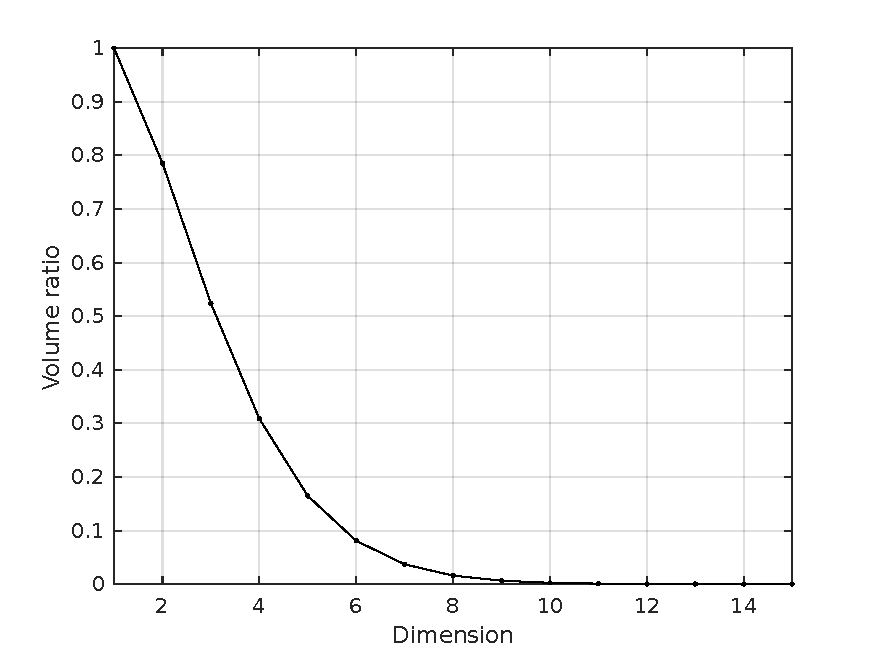
\includegraphics[scale=0.7]{hyper-objects.pdf}
	\caption{The volume ratio of a unit hyper sphere, $2\pi^{d/2}r^d/d/\Gamma(d/2)$, inside a unit hyper cube, $(2r)^d$, as a function of dimension, $d$. This example is inspired by Marko Laine.}
	\label{hyper-objects}
\end{figure}

For a likelihood distribution over a sparse high dimensional space, the majority of the space will be extraordinarily empty - i.e. with very low probability. Considering probability is a value between 1 and 0, that means a lot of parameter space will have a liklihood very close to 0. Given this circumstance it is essential to be able to accurately compute and compare extremely small probability values. The risk of improper evaluation and comparison is erraneious steps in algorithms and a divergence from the posterior the algorithm is supposed to be sampling. In short your solution will be wrong. \\

How to overcome this issue? The solution is to compute the natural logarithm of the likelihood. Figure \ref{nat-log} shows taking the natural logarithm of probability values. The result is very small probability values become very large negative numbers.

\begin{figure}[H]
	\centering
	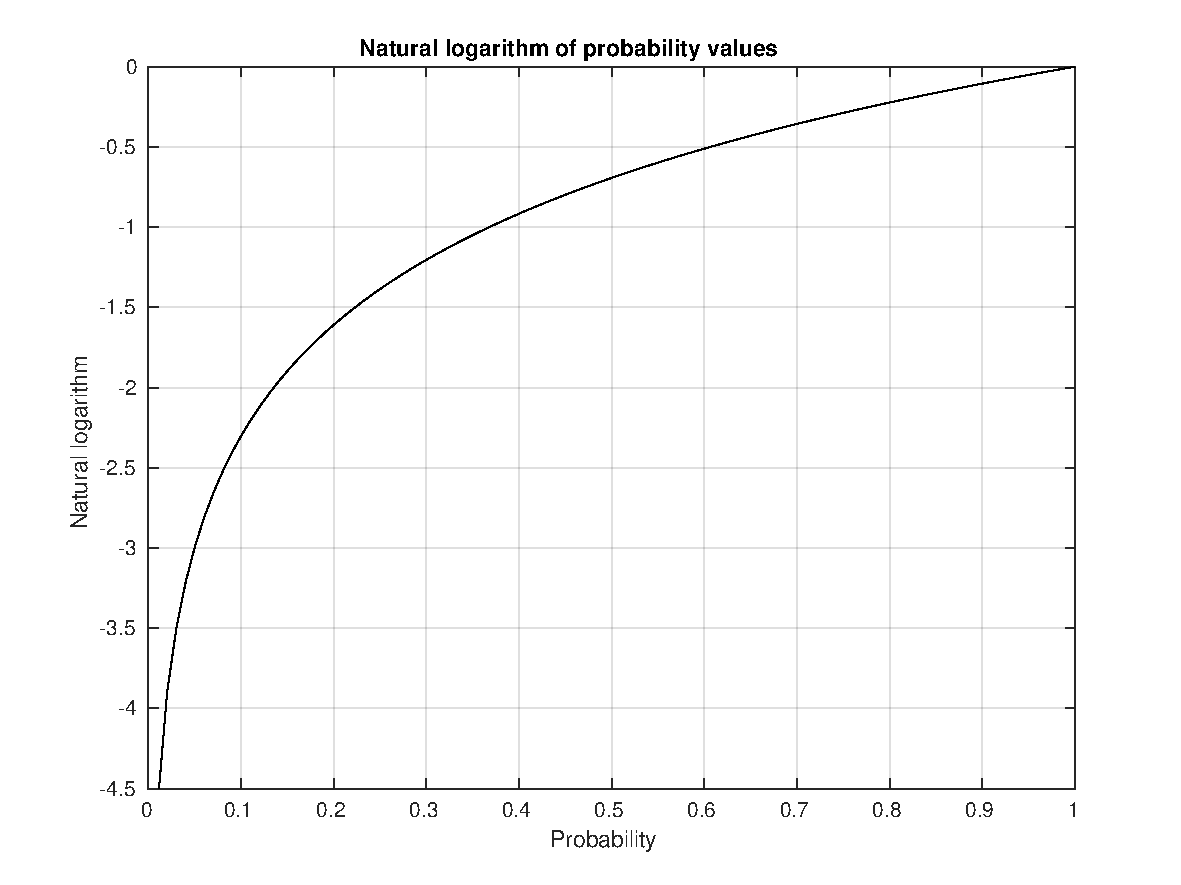
\includegraphics[scale=0.7]{nat-log.pdf}
	\caption{The natural logarithm of probability values}
	\label{nat-log}
\end{figure}

These very large negative numbers transform a very small value, close to or crossing the limits of CPU memory, into a large number which can be easily stored. \\

For a Gaussian likelihood, taking the natural logarithm...

